\section{Stime dei costi}
Stimare i costi è considerata un'attività molto complicata.
I costi possono provenire da diverse fonti:
\begin{itemize}
    \item strutture: uffici, energia
    \item risorse informatiche: hw e sw di sviluppo
    \item materiali di consumo: carta, dischi
    \item personale di supporto: segreteria, amministrazione
    \item personale tecnico: programmatori, tecnici, manager
\end{itemize}
Questi sono tutti costi di diverse entità (più grandi e più piccoli), che vengono poi ammortizzati. Alcuni costi sono fissi (non dipendono dal progetto), altri invece, come il personale tecnico, variano in base al progetto.\\
Il costo del tempo non è un costo assoluto, ma lo devo relazionare alla produttività del personale.\\
I costi sono influenzati dalla produttività, ma cosa influenza la produttività?
\begin{quote}
    "A multitude of factor influence developer productivity"
\end{quote}
Nelson-Jones identifica 250 aspetti che possono influenzare la produttività di un team di sviluppo. Tra i principali:
\begin{itemize}
    \item Numero di istruzioni da codificare: la dimensione e la complessità del progetto influenzano il tempo
    \item Capacità, motivazioni, coordinamento personale 
    \item Complessità dell'applicazione
    \item Stabilità di requisiti: cambiare requisiti diminuisce la produttività, anche perché è lavoro inutile che non può essere fatturato
    \item Prestazioni o qualità richieste
    \item Strumenti di sviluppo usati
    \item ...
\end{itemize}
Dobbiamo quindi migliore la produttività, diminuire i tempi e i costi.\\ I modi con cui posso stimare i costi possono essere:
\begin{itemize}
    \item Stime umane, in cui applico dei ragionamenti
    \begin{itemize}
        \item Legge di Parkinson sul lavoro
        \item Price to win
        \item Esperti
        \item Per analogia
    \end{itemize}
    \item Stime automatizzate
    \begin{itemize}
        \item algoritmiche: applicazione di qualche algoritmo
        \item machine learning: tecniche di intelligenza artificiale in cui si passa in input una serie di dati e si spera che tiri fuori una stima più o meno azzeccata.
    \end{itemize}
\end{itemize}

\subsection{Legge di Parkinson}
Il costo dipende dalle risorse disponibili. Come per i gas anche "Il lavoro si espanderà fino a riempire tutto il volume". In termini di stima dei costi vuol dire prendere ciò che ho disposizione e occuparlo tutto. È una visione pessimista, poiché serve tutto, ma allo stesso tempo ottimista, poiché so che basta. Una stima di questo genere, però, rende difficile fare una previsione ragionevole.

\subsection{Price to win}
Il costo è quanto il cliente è disposto a spendere (sia soldi che tempo). Vantaggio è che si ottiene il lavoro (facendo il prezzo migliore tra i concorrenti, prezzo che il cliente è disposto a pagare), svantaggio è che non si ha nessuna garanzia sul lavoro (potrei farlo male).\\
Potrebbe anche andare bene se è possibile ricontrattare i requisiti a posteriori e se è possibile lo sviluppo incrementale

\subsection{Esperti esterni}
Molto spesso quello che si fa è chiedere a esperti esterni. Si fa un primo studio di fattibilità esternamente alla ditta, per non perdere risorse e avere costi precisi. Non è una tecnica, ma una prassi comune.\\
Si delega la responsabilità ad altri per diversi motivi: sono più bravi, maggiore conoscenza del dominio, non tolgono persone interne da attività più importanti, ci danno il risultato entro una certa scadenza. \\
Ma come fanno gli esperti a fare le stime?

\subsection{Stima per analogia}
Si cerca di confrontarlo con un progetto precedente di cui la quantità di lavoro necessaria (mesi-uomo) e i tempi di sviluppo (mesi) sono noti.
Si usano coefficienti per gli scostamenti (più grande di, maggiore esperienza di, riuso..). È un metodo top-down dove si prende il progetto nel suo insieme e successivamente si suddivide la spesa.

\begin{figure}[H]
	\centering
	 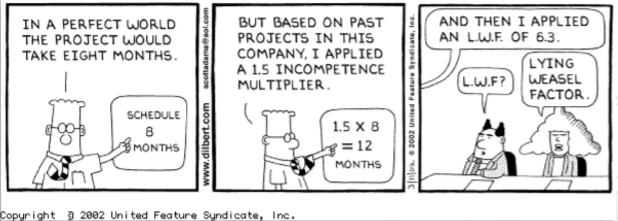
\includegraphics[width=\linewidth]{img/stimecosti.png}
	 \caption{Legge di DeMarco-Glass: Most cost estimates tend to be low}
\end{figure}
\noindent Nel momento in cui usiamo analogia possiamo basare le nostre stime su diversi fattori:
\begin{itemize}
    \item \textbf{Stima basata su dimensione del codice}: si basa sulla portata del progetto, ossia quante cose voglio che ci siano. Più cose ci sono, più devo scrivere. Piuttosto che parlare di righe di codice (che possono essere imprecise per diversi fattori), sarebbe più utile parlare di funzionalità implementate. Quindi si scompone funzionalmente il progetto e si identificano i componenti da sviluppare. Di questi si effettua una stima della dimensione. È una tecnica bottom-up: ricomponiamo la spesa totale a partire dalle singole funzionalità. Maggiore è la scomposizione (e maggiore è il dettaglio in cui si scende), minore è la difficoltà di stima dei singoli componenti
    \item \textbf{Stima basata su quantità di lavoro}: si scompone il progetto secondo una logica operativa (per fasi) e funzionale (componenti), si stima il tempo necessario per svolgere le singole fasi per il determinato componente, tecnica bottom-up.
\end{itemize}
Questi sono dei metodi umani, se vogliamo cercare di automatizzare dobbiamo cercare di trasformare in numeri:
\begin{itemize}
    \item \textbf{Produttività}: LineeCodice/MeseUomo
    \item \textbf{Qualità}: Errori/LineeCodice
    \item \textbf{Costo Unitario}: CostoTotale/LineeCodice
\end{itemize}
Queste possono essere misurate su progetti passati, posso quindi avere una base di conoscenza per ragionare sul futuro.\\
Tra le principali tecniche di stime automatizzate (algoritmiche) troviamo:
\begin{itemize}
    \item Bohem: COCOMO, COCOMO2
    \item Putnam: SLIM (Software Life Cycle Management)
\end{itemize}

\subsection{COCOMO}
COCOMO è una tecnica degli anni 80, sviluppata quando il software veniva scritto da aziende organizzate col modello a cascata. Al giorno d'oggi non rispetta quella che è stata l'evoluzione del software, per cui c'è stata anche una sua evoluzione: COCOMO 2. \\
COCOMO assume un modello cascata a 4 fasi sequenziali: 
\begin{enumerate}
    \item pianificazione e analisi requisiti
    \item progetto
    \item sviluppo
    \item integrazione e testing
\end{enumerate}
 Parte dalla misurazione di casi reali e cerca di estrarre delle formule che vadano a mappare quelli che sono i risultati. Stima i nuovi input, applica la formula e ottiene i risultati. \\

COCOMO caratterizza i progetti in base a una dimensione e ad ogni dimensione corrisponde una tipologia di formule. Le applicazioni possono essere:
\begin{itemize}
    \item \textbf{semplici}:  piccole applicazioni per cui il team è già ferrato e sa quali sono le problematiche che possono presentarsi
    \item \textbf{intermedie}: applicazioni in cui ci possono essere parti di codice in cui non ho nessuna esperienza e posso fare scelte (anche architetturali) sbagliate, accorgendomene tardi
    \item \textbf{complesse}: vincoli real-time, hardware, specifiche... Fattori esterni che complicano la scrittura dell'applicazioni
\end{itemize}
E a partire da queste COCOMO fornisce tre modelli:
\begin{itemize}
    \item \textbf{Base}: dipende solo dalla stima delle linee di codice
    \item \textbf{Intermedio}: aggiunge 15 fattori correttivi legati alle caratteristiche del progetto e permette di effettuare una stima dei singoli componenti
    \item \textbf{Avanzato}
\end{itemize}
\subsubsection{Modello base}
MesiUomo = \(aLOC^b\) \\
MesiSviluppo = \(cMesiUomo^d\)\\
dove \textit{a, b, c, d} sono parametri che variano in base alla complessità dell'applicazione (con b > 1, d < 1)\\
\begin{tabular}{ |c|c|c|c| } 
    \hline
    \textbf{Parametro} & \textbf{Semplice} & \textbf{Intermedia} & \textbf{Complessa} \\
    \hline
    a & 2.40 & 3.00 & 3.60 \\ 
    b & 1.05 & 1.12 & 1.20 \\ 
    c & 2.50 & 2.50 & 2.50 \\ 
    d & 0.38 & 0.35 & 0.32 \\ 
    \hline
\end{tabular}
\\\\Al crescere del progetto ha senso inserire nuove persone e impiegarci meno tempo.  
\begin{figure}[H]
	\centering
	 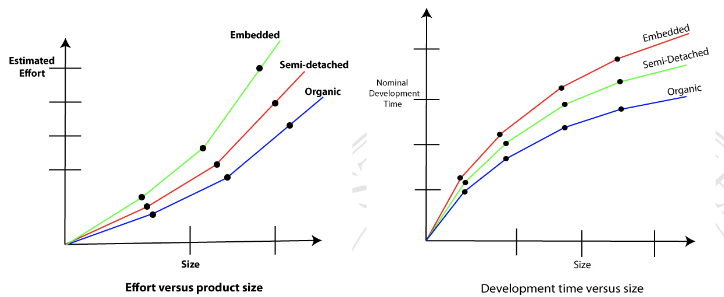
\includegraphics[width=\linewidth]{img/cocomoandamenti.png}
	 \caption{COCOMO andamenti}
\end{figure}
\noindent Con effort (MesiUomo) e development time (MesiSviluppo)  ottengo una nuova misura: il dimensionamento del team. Quante persone devo metterci a lavorare?\\
\begin{center}
 Dimensione = \(\frac{MesiUomo}{MesiSviluppo}\).\\   
\end{center}

\noindent COCOMO non vede quindi il numero di componenti del team come fattore su cui giocare per accelerare il progetto, ma come misura derivata.

\subsubsection{Modello intermedio}
Aggiunge 15 fattori correttivi da considerare:
\begin{itemize}
    \item Legati al prodotto
    \begin{itemize}
        \item affidabilità richiesta
        \item dimensione database
        \item complessità
    \end{itemize}
    \item Legati alle macchine
    \begin{itemize}
        \item efficienza richiesta
        \item memoria richiesta
        \item variabilità ambiente sviluppo
        \item tempi di risposta
    \end{itemize}
    \item Legati al progetto
    \begin{itemize}
        \item tecniche di programmazione avanzate
        \item strumenti avanzati
        \item tempi di sviluppo stretti
    \end{itemize}
    \item Legati al personale
    \begin{itemize}
        \item esperienza analisi
        \item esperienza di dominio
        \item esperienza sviluppo
    \end{itemize}
\end{itemize}
MesiUomo = \(aLOC^b\Pi c_j\) \\
MesiSviluppo = \(cMesiUomo^d\) \\

\noindent dove \(\Pi c_j\) è la produttoria dei coefficienti correttivi e a,b non sono più quelli di prima. LOC dovrebbe essere calcolato a partire dai componenti e non solo dalla stima totale. Questo consente di ottenere risultati più fini.

\subsection{COCOMO 2}

Tiene conto dei nuovi modo di sviluppare software (diversi dal modello a cascata) e usa formule diverse. In particolare tiene conto di:
\begin{itemize}
    \item Prototipizzazione
    \item Riuso
    \item COTS (commercial off the shell)
\end{itemize}
Ha diverse formule a seconda del momento della stima:
\begin{itemize}
    \item prime fasi e prototipizzazione
    \item fase di progettazione
    \item fase successiva alla definizione dell'architettura
\end{itemize}

\subsection{Stime automatizzate: Machine Learning}
Diamo in pasto ad un algoritmo una grande quantità di dati anziché fare un fitting su una funzione, che è una grossa approssimazione, ed è il motivo per cui si vanno ad inserire tutti i fattori correttivi. \\
Queste tecniche sono più efficienti avendo però una base di dati sufficiente.
\begin{itemize}
    \item Neural Networks
    \item Fuzzy Logic
    \item Case-Based Reasoning
    \item Analogy
    \item Rule-Based
    \item Regression Trees
    \item Hybrid System
\end{itemize}

\subsection{Stime collettive/condivise}

Fino ad ora si è parlato di un solo stimatore, ma nella pratica per diversi motivi si cerca di ottenere delle stime:
\begin{itemize}
    \item collettive: tanti individui che decidono separatamente danno una stima migliore di quella di un singolo esperto, perché diverse persona lasciano sfuggire meno considerazioni
    \item condivise: si fanno mettere d'accordo le diverse stime ed iterativamente si arriva ad una stima più o meno condivisa.
\end{itemize}
Nei modelli agili la responsabilità della stima passa dai manager (imposizione dall'alto) a team sviluppatori (autodeterminazione).  Il risultato finale dev'essere condiviso e accettato da tutti gli elementi del team, indipendentemente da chi la farà.\\
Abbiamo diverse tecniche che si occupano di stime condivise e collettive:
\begin{itemize}
    \item Planning Poker
    \item Team Estimation Game
    \item \#NoEstimate
\end{itemize}

Ci sono due problemi principali che un metodo di stima condivisa deve affrontare:
\begin{itemize}
    \item effetto folla, si perde tempo per troppa comunicazione
    \item effetto ancora, quando arrivano i primi pezzi di informazione (ad esempio stime da un'altra persona), non si riesce più a ragionare per termini assoluti, ma per termini relativi a quel primo elemento. 
\end{itemize}

\begin{figure}[H]
	\centering
	 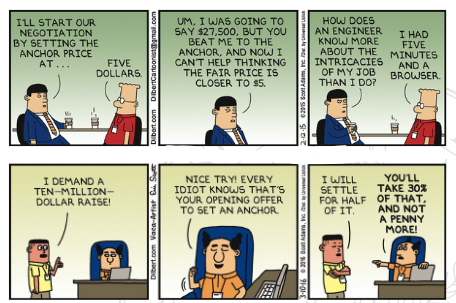
\includegraphics[scale=0.7]{img/effettoancora.png}
	 \caption{Effetto ancora}
\end{figure}

\subsubsection{Planning Poker}
\begin{enumerate}
    \item Si presentano brevemente le carte
    \item Il team può fare domande, richiedere chiarimenti e discutere per chiarire assunzioni e rischi
    \item Ogni componente sceglie una carta del poker rappresentante la propria stima. L'unità di misura di queste carte può variare e sicuramente non è lineare. Le unità di misura sono unità di misura ideali, sono numeri, non grandezze dimensionate. 
    \item Le carte vengono girate contemporaneamente (per eliminare l'effetto ancora)
    \item Chi ha espresso le stime più basse e più alte ha tot tempo per spiegare le sue motivazioni e cercare di convincere gli altri.
    \item Si ripete la votazione fino a quando si raggiunge l'unanimità.  In 3-4 iterazioni, la cosa dovrebbe convergere. Se non converge, vuol dire che la fase di chiarificazione iniziale non è stata sufficiente. A questo punto il coordinatore gestisce la cosa in qualche modo.
\end{enumerate}
Nelle metodologie si parla sempre e solo di storie. Non si vende un prodotto, si vende tempo. Rendo il più produttivo possibile quel periodo di tempo per far quelle cose che per il cliente sono importanti. Poi o si interrompe e si consegna (ad ogni consegna c'è qualcosa che ha valore per l'utente), o si va avanti a fare un'altra cosa, vendendo altro tempo. \\
Questa tipologia di contratto ha più probabilità di non fallire, rispetto ad un contratto a prodotto. È più difficile contestarlo.

\subsubsection{Team Estimation Game}
Composto da 3 fasi coglie di più gli aspetti critici di ancoraggio e comunicazione.\\ È molto più efficiente per stimare tante carte.
\begin{enumerate}
    \item \textbf{Valutazione comparativa}: ad un tavolo si mettono in fila i developer. C'è una pila delle stories. Il primo prende la prima carta, la legge ad alta voce, la piazza al centro del tavolo e a questo punto si mette in coda. Il (nuovo) primo prende la carta dalla pila e decide lui in autonomia se è più semplice, più complicata o equivalente a quella che c'è già sul tavolo, mettendola a sinistra, destra o sotto. Il prossimo può prendere una nuova carta e posizionarla rispetto a tutto il gruppo o tra due gruppi, oppure ancora sotto. Altrimenti può spostare una carta già posizionata, motivando. Se non ci sono carte in pila e non ce n'è nessuna che vuole spostare, passa. Itera finché non ci sono più carte e non c'è nessun developer che vuole spostare una carta. C'è un effetto ancora diverso, perché non è su un valore, ma su una relazione. Non è significativo. La comunicazione non è globale, ma è solo di colui che sposta.
    \item \textbf{Quantificazione delle distanze}: di nuovo ci si mette in coda davanti al tavolo. Carte disposte a colonne. Ho un mazzo tipo quello del planning poker che ha i valori possibili. Queste carte sono ordinate. Si prende la prima (di solito 2, per avere margine sotto). Ognuno pesca una carta e decide su quale colonna metterla. Arriva un altro dev e può o prendere una carta e metterla su una colonna (alcune colonne possono anche essere saltate), oppure propone uno spostamento in una nuova posizione di una delle carte oppure ancora, se va tutto bene, passa. Si ripete finché son finite le carte. Si può anche decidere che non ci sia alcuna storia che corrisponda a quel valore. Le colonne senza valore vengono assimilate alla colonna alla loro sinistra. A questo punto ogni colonna ha un valore. Non ha ancora una scala effettiva.
    \item \textbf{Scala assoluta}:Prendo una delle carte a cui ho dato valore più semplice (2) e stimo a quante ore/uomo corrisponde. Dopodiché si fa una proporzione con tutte le altre. A questo punto abbiamo trovato una scala.
\end{enumerate}
La terza fase dopo la prima volta che si esegue team estimation game si perde. \\
Si lavora, avendo iterazioni corte, basate sul concetto di velocity: capacità osservata nell'iterazione precedente di completare lavori da parte del team. \\ Nell'iterazione dopo si danno le stime con gli stessi valori, non importa quale sia la scala. Nell'iterazione successiva posso anche adattare le stime fino a convergere con quella che è la velocità effettiva delle persone. \\
Ogni team ha un suo numero che non è confrontabile con quello stimato dagli altri team. Non dev'essere usato come metodo di valutazione, poiché possono corrispondere a scale diverse. \\
Non si considerano storie non finite. \\
Non deve nemmeno essere imposta dall'esterno.


\subsubsection{\#NoEstimate}
Nei metodi agili non c'è un commitment totale, è un'indicazione di ciò che riesco fare. È ammesso sbagliare, si adatta alla velocity pian piano. \\
Non essendo così rigidi, perchè non eliminare la stima? Non è particolarmente importante per l'utente. Non perdiamo tempo a fare stime. \\
Questo funziona per team maturi perché splittando le storie, si ottengono storie della stessa dimensione, aiutando l'omogeneità. In un certo senso si fanno stime in maniera inconscia.